% ---
% JAVA ORACLE EVENT PROCESSING (OEP)
%
% ---

\chapter{Java Oracle Event Processing}

Este capítulo tem como objetivo demonstrar a plataforma \textit{Java Embedded}
- \textit{Java Oracle Event Processing} (\textit{OEP}).

\section{Instalação}

A plataforma de prototipagem deve estar operacional com o sistema operacional
\textit{Linux} e a plataforma \textit{Java 8}, no caso de estudo a plataforma
\textit{Raspberry PI B+}. A figura \ref{fig:oep/configuracao} apresenta as
configurações do sistema em estudo.

\begin{figure}[H]
    \centering
    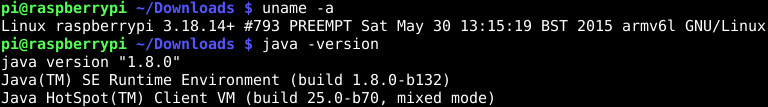
\includegraphics[width=0.7\linewidth]{figuras/java/configuracao}
    \caption{Configuração do Sistema}
    \label{fig:oep/configuracao}
\end{figure}

Para a plataforma de prototipagem é necessário a instalação do pacote
\textit{Oracle Java Embedded Suite 7.0} e \textit{Oracle Event Processing for
    Oracle Java Embedded}, necessário ter uma conta no site da \textit{Oracle}
para realizar o \textit{download}.

Transfira os arquivos \newline
\verb|jes-7.0-ga-bin-b11-linux-arm-runtime-15_nov_2012.zip|
, \newline
\verb|jes-7.0-ga-b11-linux-samples-15_nov_2012.zip|
e \newline
\verb|ofm_oep_embedded_11_1_1_7_1_linux.zip|
 do sistema operacional principal para o dispositivo remoto, basta utilizar o
comando \textit{SCP}:

\verb|scp </path/from/file> <user>@<address>:/path/to/destination|

Descompacte os arquivos, basta utilizar o comando \textit{UNZIP}:

\verb|unzip <file>|

\section{Aplicações para a Internet das Coisas}

O \textit{OEP} permite as aplicações na \textit{Internet} das Coisas -
\textit{Internet of Things} (\textit{IoT}), o processamento em tempo real dos
dados amostrados através dos periféricos e recursos encontrados nos
dispositivos, assim aplicando técnicas de filtragens e estatísticas para a
realização de análises.

\section{Resultados}

Os resultados demonstram a visão na qual a plataforma \textit{OEP} contribui
para o desenvolvimento de aplicações destinadas a \textit{IoT}.

\subsection{Positivos}

\begin{itemize}

    \item Grande poder de processamento, por oferecer uma gama de recursos para
    trabalhar com dados;

    \item Utilização de linguagem de consulta para a manipulação e amostragem
    dos dados;

    \item Traz a capacidade de \textit{gateway} para o dispositivo, quando
    conectado em outros dispositivos.

\end{itemize}

\subsection{Negativos}

\begin{itemize}

    \item Não possui uma interface de desenvolvimento produtiva como encontrada
    na versão tradicional através de linguagem gráfica.

\end{itemize}
